\newcommand{\package}{\emph}
\section{The model}
The model for a two protein network can be given by the system of equations:

\begin{subequations}
	\begin{align}
		\frac{dx}{dt} &= f(y) - d_1 x \\
		\frac{dy}{dt} &= g(x) - d_2 y
	\end{align}
\end{subequations}
where $x$ and $y$ are the concentration of the two proteins, $f$ and $g$ are
``repression functions'' and $d_1 x$, $d_2 y$ are positive constant describing
the protein decay.

\begin{subequations}
	\begin{align}
		f(y) &= \frac{k_1}{1+[Y]^n} \footnote{where n is greater than 1 due to
	cooperativity}\\
		g(x) &= \frac{k_2}{1+[X]^m} \footnote{where m is 
		equal to 1 due to no cooperativity}
	\end{align}
\end{subequations}

 The level of repression of $[X]$ in a ``mixed'' circuit
model is described by a Hill function, which models copperativity of binding between two
different molecular species. Using the conditions for a change in the number of
steady states derived from nullclines analysis:


\begin{subequations}
	\begin{align}
		d_1 [X] &= \frac{k_1}{1+[Y]^n}*\frac{1}{d_1} = \frac{k'_1}{1+[Y]^n}
		\footnote{with $k'_1 = \frac{k_1}{d_1}$} \label{eq:subeq1}\\ 
		y_1 &= \sqrt[n]{\frac{k'_1}{d_1 [X]}-1}\\
		d_2[Y] &= \frac{k_2}{1+[X]}*\frac{1}{d_2} = \frac{k'_2}{1+[X]^n}
		\footnote{with $k'_2 = \frac{k_2}{d_2}$} \\
		y_2 &= \frac{k'_2}{1+[X]} \label{eq:subeq2}
	\end{align}
\end{subequations}

The equations \ref{eq:subeq1} and \ref{eq:subeq2} are solved as functions of
$f(x)$ in the form $y = f(x)$.

\section{Nullcline plots}
The analysis performed in graphs \ref{fig:nullclinesplots} shows the existence
of multiple steady states, which it is the necessary condition to have a switch.
The purpose of the switch is to obtain a consisting change in the concentration
of a certain protein. The graph \ref{fig:k24} shows highly transverse
nullclines, the system can tolerate more movements of the nullclines without the
disappearance of a steady state.

\begin{figure}[h!]
  \centering
  \subfloat[$k'_2=2$]{\label{fig:k22}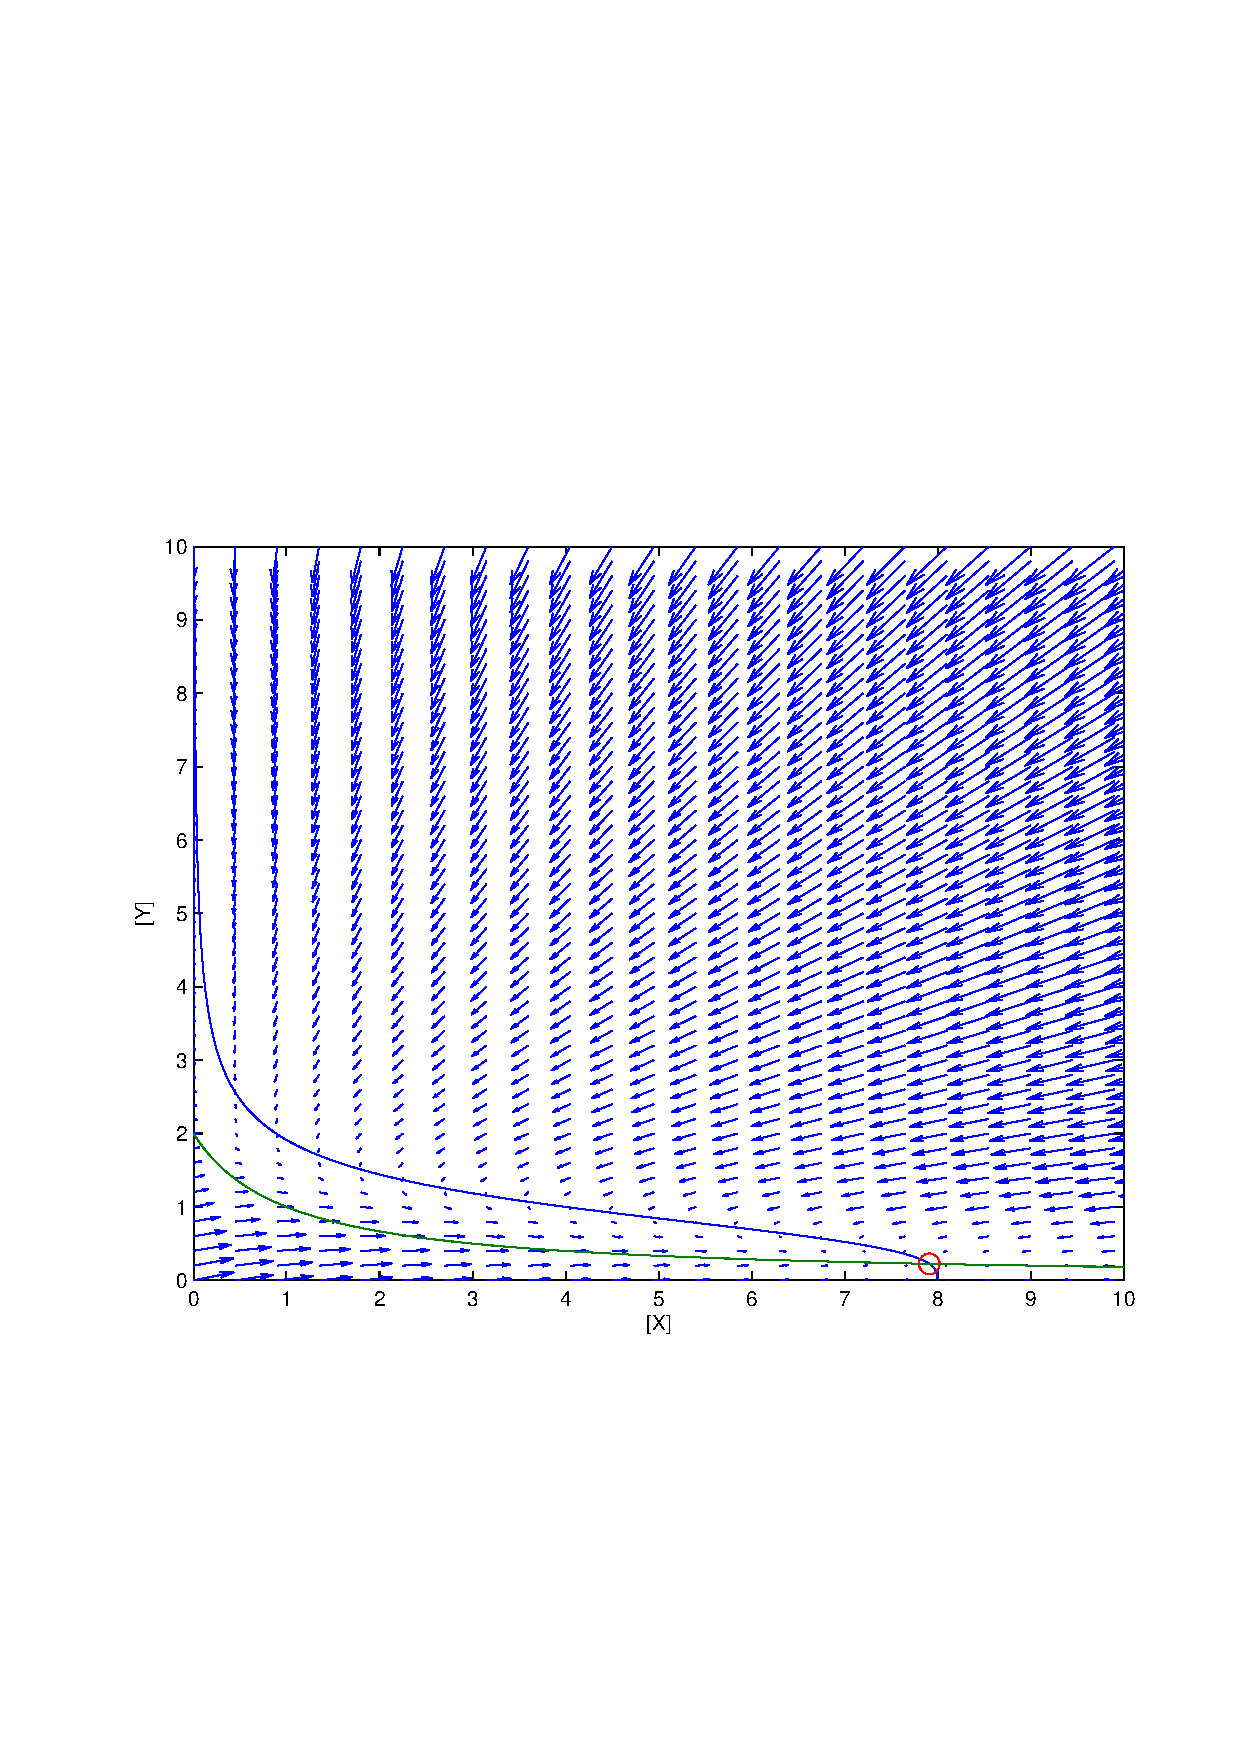
\includegraphics[height=0.55\textwidth,width=0.35\textwidth]{plot_B1}}
  ~
  \subfloat[$k'_2=4$]{\label{fig:k24}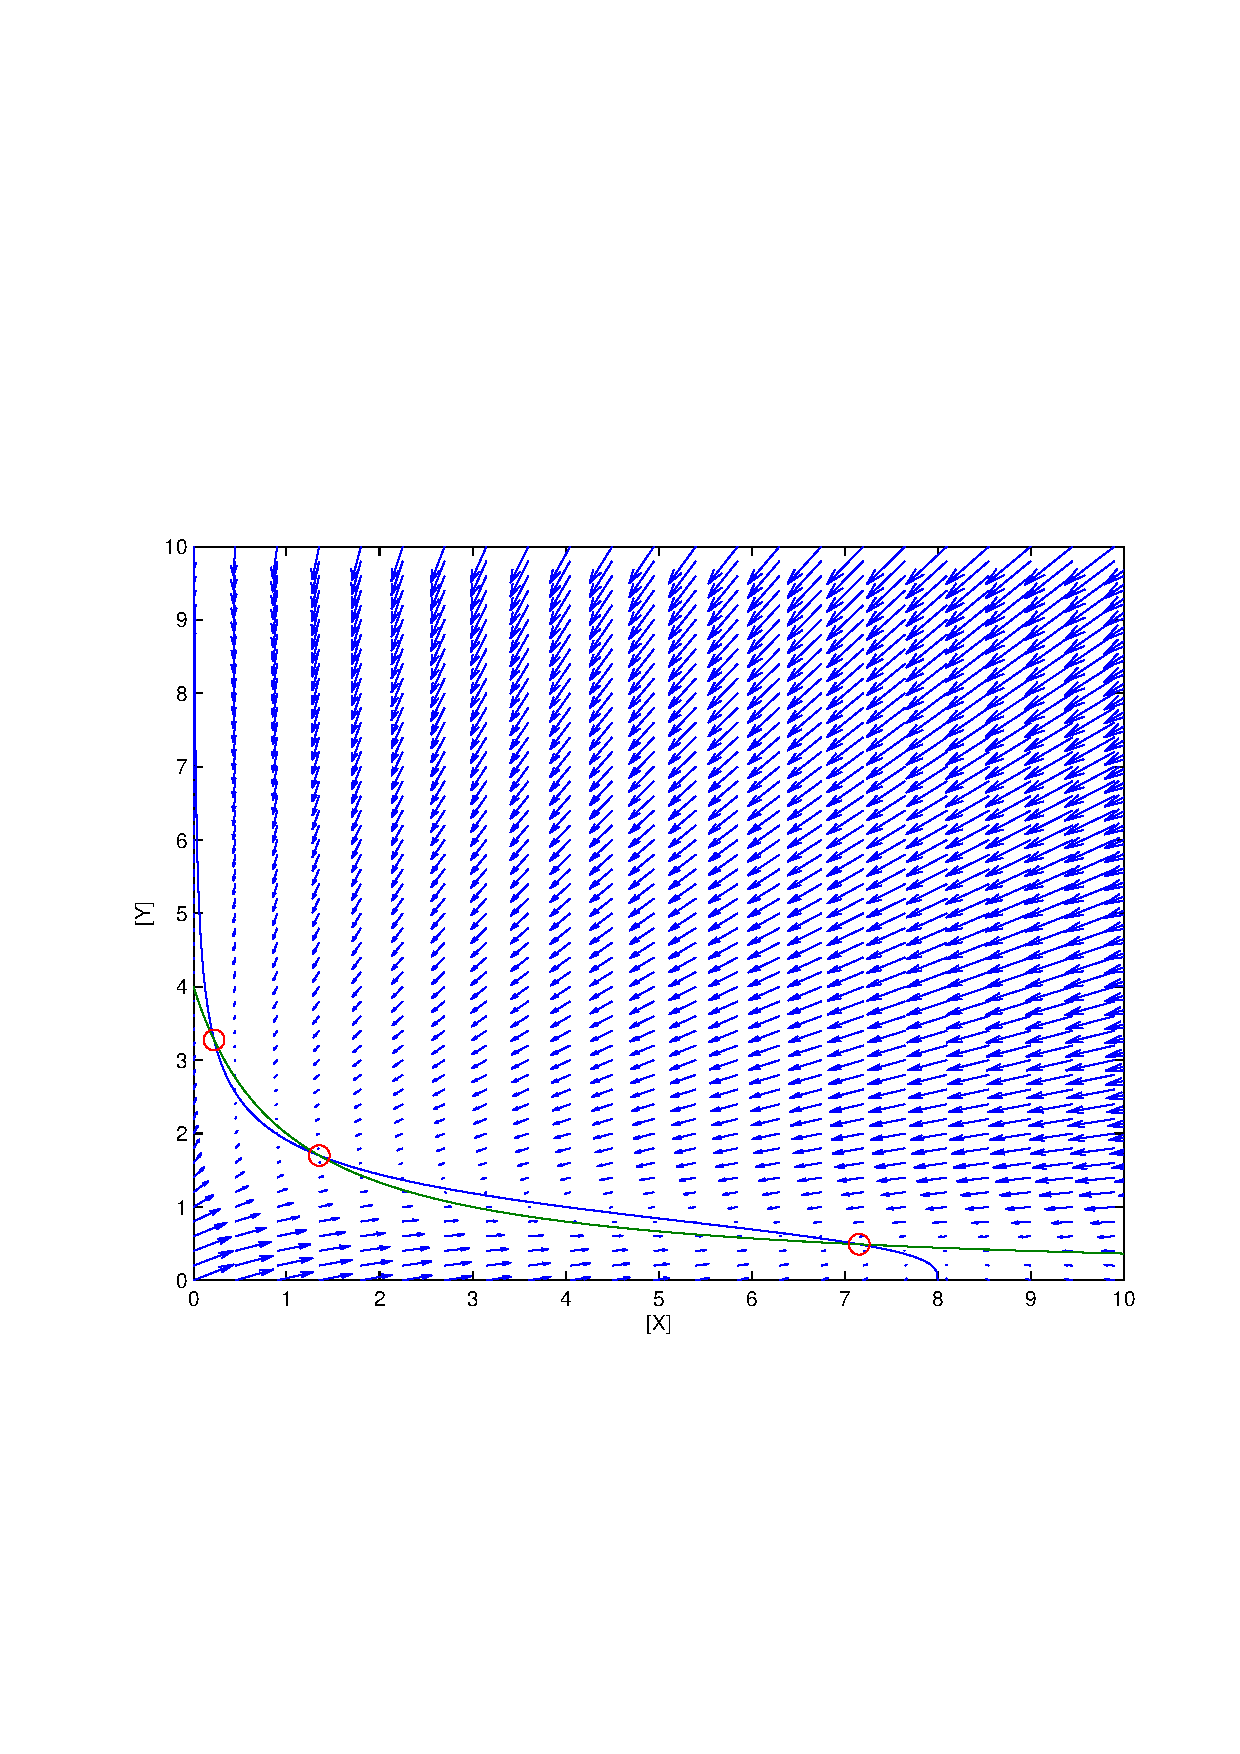
\includegraphics[height=0.55\textwidth,width=0.35\textwidth]{plot_B2}}
  ~
  \subfloat[$k'_2=6$]{\label{fig:k26}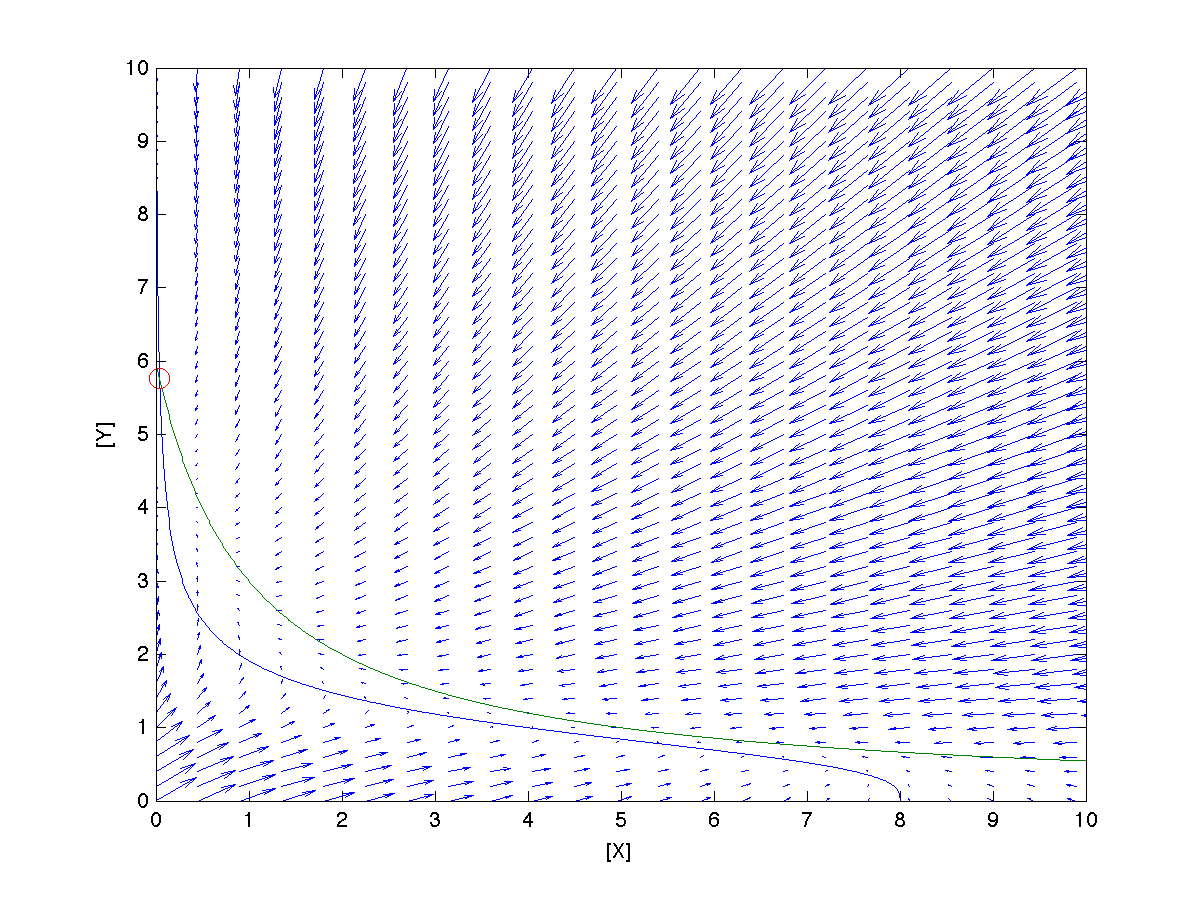
\includegraphics[height=0.55\textwidth,width=0.35\textwidth]{plot_B3}}
  \caption{Nullclines plots for the parametres $n = 3$ , $k'_1 = 8$ , $k'_2 =
  \{2,4,6\}$}
  \label{fig:nullclinesplots}
\end{figure}

Intersection of functions lines are circled in red. These points represent the
steady state at different values of the parameter $k_2$. In the graph
\ref{fig:k22} we can distinguish only one point at high concentration of protein
$Y$ as well as in the graph \ref{fig:k26} where the steady state is reached at
high concentration of $X$. The major difference is visible in the graph
\ref{fig:k24} where we clearly confirm a possible switch, due to the
presence of three steady state points.

\section{Analytic expressions for $k'_1$ and $k'_2$}

According to Matlab \emph{solve} function for the
equations:

\begin{subequations}
	\begin{align}
		e1 &: x = \frac{k'_1}{(1+y^3)}\\
		e2 &: y = \frac{k2}{(1+x)}\\
		e3 &: \delta(\frac{k_1}{(1+y^3)}, y)*\delta(\frac{k_2}{(1+x)},x) = 1
	\end{align}
\end{subequations}



we retrieve three solutions:

\begin{subequations}
	\begin{align}
		k'_1 &=\frac{(3*x^2)}{(2*x - 1)}\\ 
		k'_2 &=\left(\frac{(x + 1)}{(2*x - 1)}\right)^\frac{1}{3}*(x + 1)\\
		y &= \left(\frac{(x + 1)}{(2*x - 1)}\right)^\frac{1}{3}
	\end{align}
\end{subequations}

\section{Cooperativity plot}


\begin{figure}[h]
  	\centering
    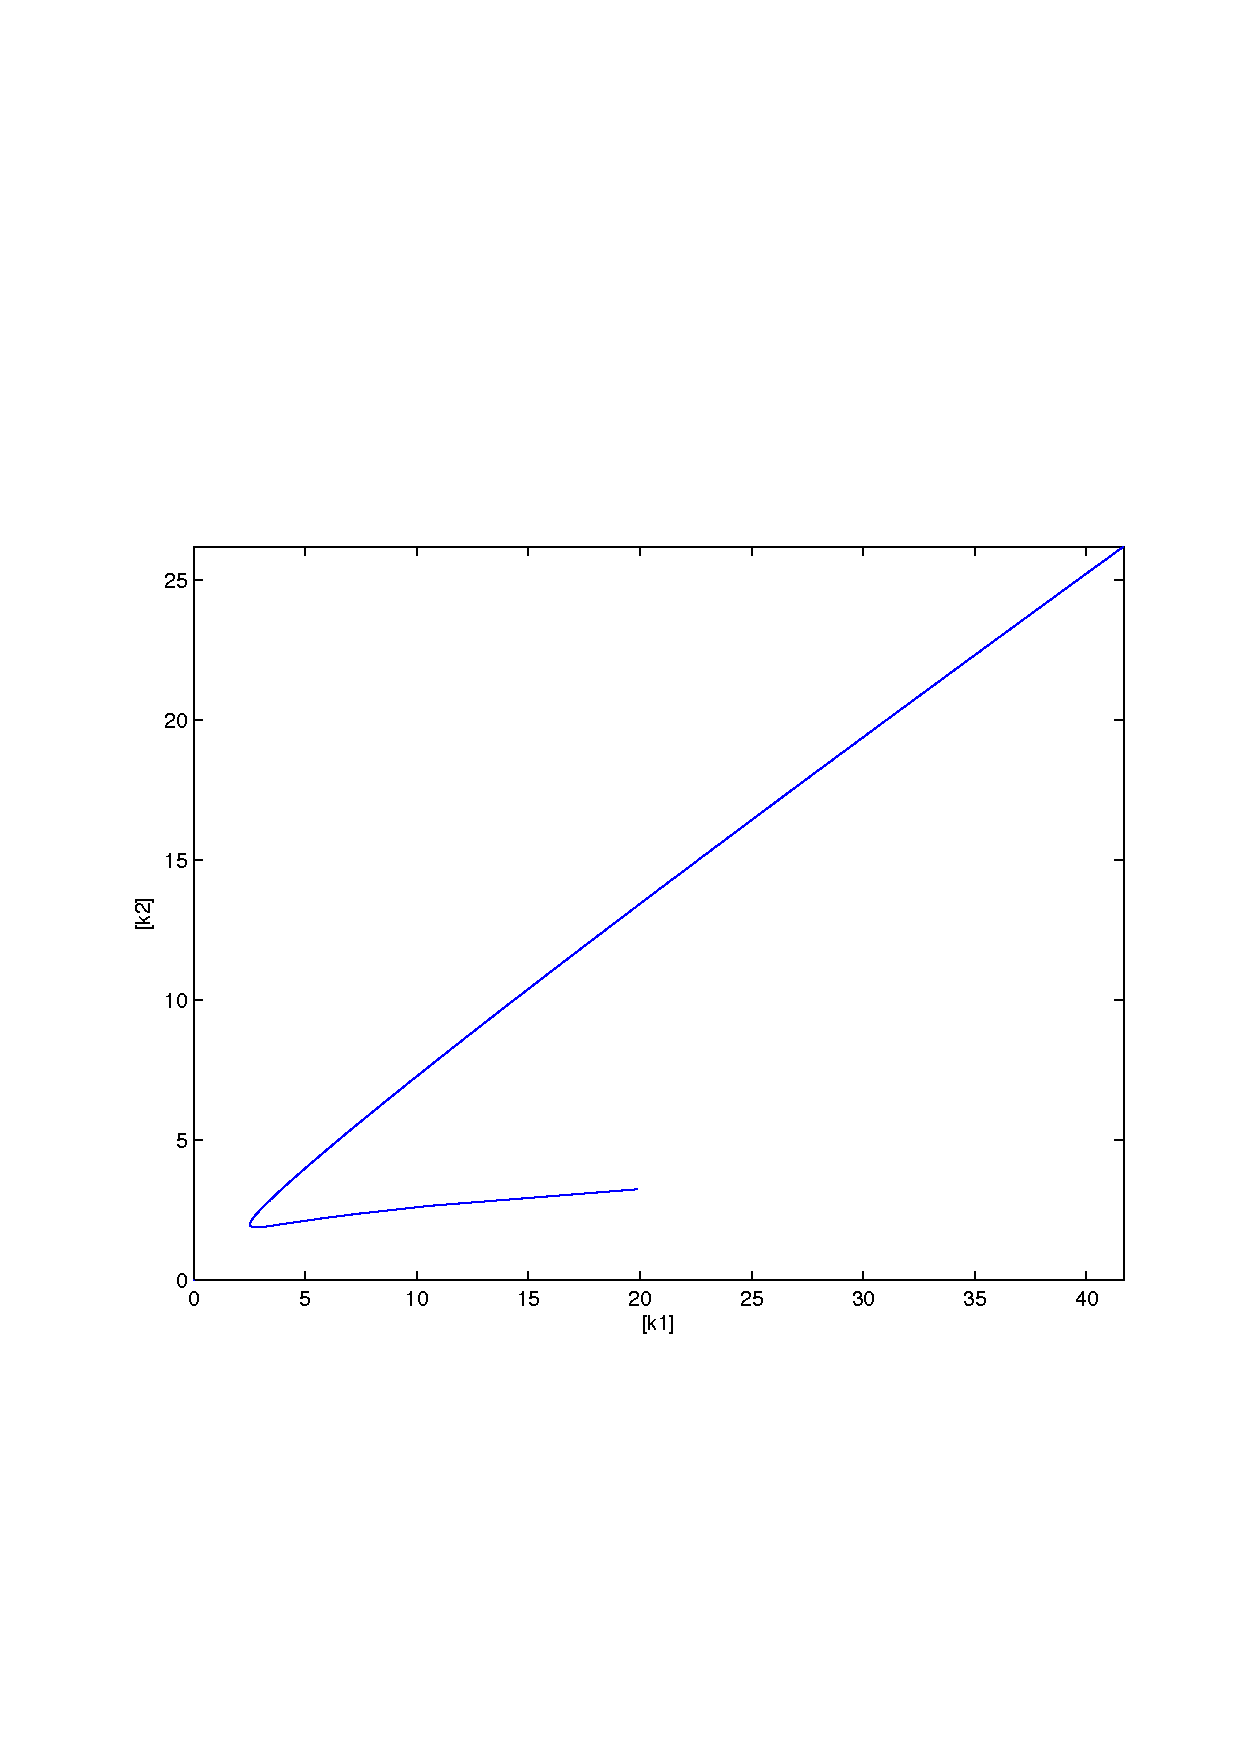
\includegraphics[width=0.85\textwidth]{plot_D0}
    \caption{Values of the parameter $k'_1$ and $k'_2$ needed for a working switch
 	for particular values of the exponent $n$ in the Hill function \ldots}
	\label{fig:bifurcatingplot}
\end{figure}
  


